\begin{figure}[H]
    \centering
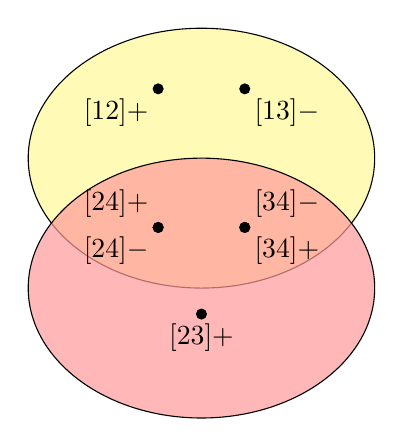
\begin{tikzpicture}
    \def\side{1.1}
    
    \begin{scope}[fill opacity=0.7]
    \filldraw[fill=yellow!40] (0,0) ellipse [x radius=2*\side, y radius=1.5*\side];

    \filldraw[fill=red!40] (0,-1.5*\side) ellipse [x radius=2*\side, y radius=1.5*\side];
    \end{scope}

   % \node (143) at (-0.5*\side, -1.3*\side) {};

    \fill (-0.5*\side, -0.8*\side) circle (2pt) node [above left] {$[24]+$}; 

    \fill (0.5*\side, -0.8*\side) circle (2pt) node [above right] {$[34]-$}; 

    \fill (-0.5*\side, -0.8*\side) circle (2pt) node [below left] {$[24]-$}; 

    \fill (0.5*\side, -0.8*\side) circle (2pt) node [below right] {$[34]+$}; 

    \fill (0.5*\side, 0.8*\side) circle (2pt) node [below right] {$[13]-$};

    \fill (-0.5*\side, 0.8*\side) circle (2pt) node [below left] {$[12]+$};

    \fill (0, -1.8*\side) circle (2pt) node [below] {$[23]+$};
\end{tikzpicture}
\caption{The weighted oriented hypergraph $\widetilde{\KK}$,
each vertex has weight $1$, 
the yellow hyperedge has weight $1/2$, 
and the red hyperedge has weight $1$.
The Laplacian $\Delta_0^{\widetilde{\KK}}$ is equal to the up persistent Laplacian $\Delta_{1, \mathrm{up}}^{\KK, \LL}$ with respect to $\KK\hookrightarrow \LL$ associated with Figure \ref{fig_simplicial_cmplexes}.}
\label{fig_hg_ex_1}
\end{figure}